

%----------------------------------------------------------------------------------------
%	PACKAGES AND OTHER DOCUMENT CONFIGURATIONS
%----------------------------------------------------------------------------------------

\documentclass[12pt]{article}

\usepackage{polski}
\usepackage[polish]{babel}
\usepackage[utf8]{inputenc}
\usepackage{datetime}
\usepackage{graphicx}
\usepackage{tikz} 
\usepackage{amsmath}  
\usepackage{epstopdf}
\usepackage{float}
%\usepackage[colorlinks=true]{hyperref}
%\usepackage[all]{hypcap}
%\usepackage{showframe}
\usepackage{geometry}
 \geometry{
 a4paper, 
 left=30mm,
 right=30mm,
 top=30mm,
 bottom=30mm,
 }
 
\newdate{create_date}{27}{03}{2014}

%----------------------------------------------------------------------------------------

%----------------------------------------------------------------------------------------
% TIKZ PACKAGES
%----------------------------------------------------------------------------------------

\usetikzlibrary{arrows}

%----------------------------------------------------------------------------------------

\begin{document}

\begin{titlepage}

\newcommand{\HRule}{\rule{\linewidth}{0.5mm}}
% Defines a new command for the horizontal lines, change thickness here

\center
% Center everything on the page
 
%----------------------------------------------------------------------------------------
%	LOGO SECTION
%----------------------------------------------------------------------------------------


\includegraphics[width=6cm]{../res/img/logo.png}\\[1cm]
% Include a department/university logo - this will require the graphicx package
 
%----------------------------------------------------------------------------------------
 
%----------------------------------------------------------------------------------------
%	HEADING SECTIONS
%----------------------------------------------------------------------------------------

\textsc{\LARGE Akademia Górniczo-Hutnicza \\[0.2cm]
im. Stanisława Staszica w Krakowie}\\[1.5cm]
% Name of your university/college

\textsc{\Large Podstawy Automatyki}\\[0.5cm]
% Major heading such as course name

%----------------------------------------------------------------------------------------
%	TITLE SECTION
%----------------------------------------------------------------------------------------

\HRule \\[0.5cm]
{ \huge \bfseries Dyskretne układy regulacji \\[0.3cm] oraz \\[0.5cm] Analiza
serwomechanizmu \\[0.2cm] przekaźnikowego z wykorzystaniem płaszczyzny
fazowej}\\[0.3cm]
% Title of your document
\HRule \\[1.5cm]
 
%----------------------------------------------------------------------------------------
%	AUTHOR SECTION
%----------------------------------------------------------------------------------------

% \begin{minipage}{0.4\textwidth}
% \begin{flushleft} \large
% \emph{Author:}\\
% Konrad \textsc{Adasiewcz} % Your name
% \end{flushleft}
% \end{minipage}
% ~
% \begin{minipage}{0.4\textwidth}
% \begin{flushright} \large
% \emph{Supervisor:} \\
% dr inż. Paweł \textsc{Rotter} % Supervisor's Name
% \end{flushright}
% \end{minipage}\\[4cm]

% If you don't want a supervisor, uncomment the two lines below and remove the section above
\flushright
\Large \emph{Autorzy:}\\
Konrad \textsc{Adasiewcz}\\[0.1cm] % Your name
Michał \textsc{Maciejewski}\\[3cm] % Your name

%----------------------------------------------------------------------------------------
%	DATE SECTION
%----------------------------------------------------------------------------------------
Data wykonania ćwiczenia: \\
{\large \displaydate{exercise_date}}\\[1cm]


\vfill % Fill the rest of the page with whitespace

\end{titlepage}

\section{Wstęp teoretyczny}


\begin{figure}[!htb]
	\begin{center}
		\begin{tikzpicture}[scale=0.2]
	\draw[thick]				% Ground level
				 	(0,0) 	--
					(10,0) 	--
					(10,1) 	--
					(0,1)		--
					cycle ;
					
	\draw[ultra thick] 	% Spring k1
					(1,1)		--
					(1,3)		--
					(3,4)		--
					(-1,6)	--
					(3,8)		--
					(-1,10)	--
					(3,12)	--
					(-1,14)	--
					(1,15)	--
					(1,17)	;
	\draw 	(-4,9) node{\LARGE $k_1$};
					
	\draw[ultra thick] 	% Suppressor c1 1/3
					(9,1)		--
					(9,5)		;
	\draw[ultra thick] 	% Suppressor c1 2/3
					(8,14)	--
					(8,5)		--
					(10,5)	--
					(10,14)	;
	\draw[ultra thick] 	% Suppressor c1 3/3
					(9,8)	--
					(9,17)		;
	\draw 	(13,9) node{\LARGE $c_1$};
					
	\draw[thick] 				% Wheel mass
				 	(0,17) 		--
					(10,17) 	--
					(10,27) 	--
					(0,27)		--
					cycle ; 
	\draw 	(5,22) node{\LARGE $m_1$};
	
	\draw[ultra thick] 	% Spring k2
					(1,27)	--
					(1,29)	--
					(3,30)	--
					(-1,32)	--
					(3,34)	--
					(-1,36)	--
					(3,38)	--
					(-1,40)	--
					(1,41)	--
					(1,43)	;
	\draw 	(-4,35) node{\LARGE $k_2$};
					
	\draw[ultra thick] 	% Suppressor c2 1/3
					(9,27)	--
					(9,31)	;
	\draw[ultra thick] 	% Suppressor c2 2/3
					(8,40)	--
					(8,31)	--
					(10,31)	--
					(10,40)	;
	\draw[ultra thick] 	% Suppressor c2 3/3
					(9,34)	--
					(9,43)	;
	\draw 	(13,35) node{\LARGE $c_2$};
					
	\draw[thick] 				% Wheel mass
				 	(0,43) 		--
					(10,43) 	--
					(10,53) 	--
					(0,53)		--
					cycle ; 
	\draw 	(5,48) node{\LARGE $m_2$};
	
	\draw[-latex, line width=3pt]	% Axis
					(-10,0)		--
					(-10,60) node[xshift=-15pt, yshift=-23pt]{\LARGE $x$};
	\draw[line width=3pt]
					(-10,0)		--
					(-15,0)		node[left]{\LARGE $0$};
	\draw[line width=3pt]
					(-10,17)	--
					(-15,17)	node[left]{\LARGE $x_{10}$};
	\draw[line width=3pt]
					(-10,43)	--
					(-15,43)	node[left]{\LARGE $x_{20}$};
					
	\draw[thick]
					(10,0)	--
					(15,0)	node[right]{\LARGE $x_{0}$};
	\draw[thick]
					(10,17)	--
					(15,17)	node[right]{\LARGE $x_{1}$};
	\draw[thick]
					(10,43)	--
					(15,43)	node[right]{\LARGE $x_{2}$};

\end{tikzpicture}
		\caption{Kinematyczny schemat modelowanego fragmentu
		zawieszenia}\label{rys:sch}
	\end{center}
\end{figure}

Modelowany fragment zawieszenia przedstawiony jest na schemacie na rysunku
\ref{rys:sch}. Masa $m_1$ symbolizuje koło, natomiast masa $m_2$
reprezentuje ciało samochodu. Sprężyna $k_1$ i amortyzator $c_1$ reprezentują
właściwości sprężyste i tłumiące opony koła, natomiast sprężyna $k_2$ i
amortyzator $c_2$ to właściwy układ amortyzacyjny zawieszenia. $x_{10}$ oraz
$x_{20}$ to spoczynkowe wartości położenia koła i karoserii samochodu, natomiast
$x_1$ oraz $x_2$ to aktualne ich położenia, $x_0$ jest sygnałem
reprezentującym poziom nawierzchni.
 
\newpage

Siła działająca na koło wskutek sprężystości założonej nań opony wynosi:

\begin{equation*}
	F_{11} = -k_1(x_1-x_{10}-x_0)-c_1(\dot{x_1}-\dot{x_0})
\end{equation*}

Siła działająca na koło od strony masy samochodu wynosi:

\begin{equation*}
	F_{12} = -k_2(x_{20}-x_2-x_{10}+x_1)-c_2(\dot{x_2}-\dot{x_1})
\end{equation*}

Siła wywierana na samochód od strony koła jest zgodnie z trzecią zasadą dynamiki
Newtona równa:

\begin{equation*}
	F_{22} = -F_{12}
\end{equation*}

Kładąc zmienne odchyłkowe $y_2=x_2-x_{20}$ oraz $y_1=x_1-x_{10}$ i
mając na uwadze, iż $F_1=\ddot{x_1}m_1$ oraz $F_2=\ddot{x_2}m_2$ dostajemy następujący
układ równań różniczkowych:

\begin{equation}
	\begin{cases}
		\ddot{y_1}=
								-\frac{k_1+k_2}{m_1}y_1+\frac{k_2}{m_1}y_2-\frac{c_1+c_2}{m_1}\dot{y_1}
								+\frac{c_2}{m_1}\dot{y_2}+\frac{k_1}{m_1}x_0+\frac{c_1}{m_1}\dot{x_0}
								\\
		\ddot{y_2}=
								\frac{k_2}{m_2}y_1-\frac{k_2}{m_2}y_2+\frac{c_2}{m_2}\dot{y_1}
								-\frac{c_2}{m_2}\dot{y_2}						
								\\
		y=y_2
	\end{cases}
	\label{equ:uklrow}
\end{equation}

Chcąc przejść do równania stanu podstawiamy:

\begin{equation*}
	\begin{cases}
		y_3= \dot{y_1}-\frac{c_1}{m_1}x_0
								\\
		y_4=	\dot{y_2}
								
	\end{cases}
\end{equation*}

Otrzymujemy następujące równanie stanu:

\begin{equation}
	\begin{cases}
		\begin{bmatrix}
			\dot{y_1} \\
			\dot{y_2} \\
			\dot{y_3} \\
			\dot{y_4}
		\end{bmatrix} =	
		\begin{bmatrix}
			0 & 0 & 1 & 0 \\
			0 & 0 & 0 & 1 \\
			-\frac{k_1+k_2}{m_2} &
			\frac{k_2}{m_1} &
			-\frac{c_1+c_2}{m_1} &
			\frac{c_2}{m_1}\\
			\frac{k_2}{m_2} &
			-\frac{k_2}{m_2} &
			\frac{c_2}{m_2} &
			-\frac{c_2}{m_2}
		\end{bmatrix} \cdot
		\begin{bmatrix}
			y_1 \\
			y_2 \\
			y_3 \\
			y_4
		\end{bmatrix} +
		\begin{bmatrix}
			\frac{c_1}{m_1} \\
			0 \\
			\frac{k_1}{m_1}-\frac{(c_1+c_2)c_1}{m_1^2} \\
			\frac{c_1c_2}{m_1m_2}
		\end{bmatrix} \cdot
		x_0
		\\%[2cm]
		y =
		\begin{bmatrix}
			0 & 1 & 0 & 0
		\end{bmatrix} \cdot
		\begin{bmatrix}
			y_1 \\
			y_2 \\
			y_3 \\
			y_4
		\end{bmatrix} +
		0 \cdot x_0
	\end{cases}
	\label{equ:rstanu}
\end{equation} 
 
\newpage

\section{Realizacja modelu na integratorach}

\begin{figure}[!htb]
	\begin{center}
		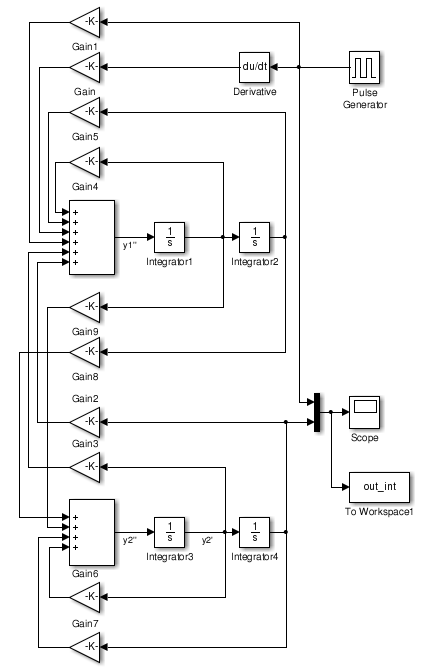
\includegraphics[width=10cm]{../res/img/integ.png}
	\end{center}
	\caption{Schemat modelu zawieszenia zrealizowany na integratorach}
	\label{rys:schd}
\end{figure}

Model zbudowany na integratorach opiera się o układ równań \eqref{equ:uklrow},
więc na podwójnym całkowaniu sygnałów $\ddot{y_1}$ oraz $\ddot{y_2}$.

\newpage

\section{Realizacja modelu na integratorach, bez członu różniczkującego sygnał
wejściowy}

\begin{figure}[!htb]
	\begin{center}
		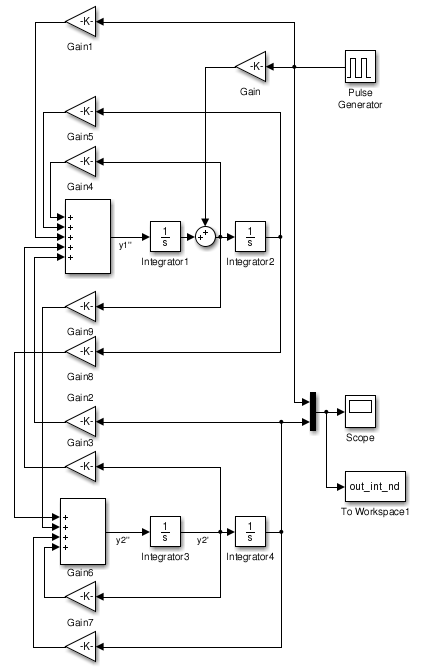
\includegraphics[width=10cm]{../res/img/integ_nd.png}
	\end{center}
	\caption{Schemat modelu zawieszenia zrealizowany na integratorach bez członu
	różniczkującego}
	\label{rys:schnd}
\end{figure}

Model zbudowany na integratorach zawiera blok różniczkujący sygnał wejściowy
gdyż potrzeba jego użycia wynika z postaci układu równań \eqref{equ:uklrow}.
Blok ten można wyeliminować korzystając z liniowości operacji całkowania. W tym celu
wpinamy sygnał $\frac{c_1}{m_1}x_0$ za integratorem sygnału $\ddot{y_1}$.

\newpage

\section{Analiza modelu}

\subsection{Parametry modeli}

Symulacje w \textsc{Simulinku} zostały przeprowadzone dla następujących
parametrów modeli: 

\begin{table}[!htb]
	\begin{center}
		\renewcommand{\arraystretch}{1.4}
		\begin{tabular}{|l|r|}
		\hline 
			$m_1$ & $90 [\textrm{kg}]$ \\
		\hline
			$m_2$ & $600 [\textrm{kg}]$ \\
		\hline
			$k_1$ & $370 [\frac{\textrm{kN}}{\textrm{m}}]$ \\
		\hline
			$k_2$ & $35 [\frac{\textrm{kN}}{\textrm{m}}]$  \\
		\hline
			$c_1$ & $100 [\frac{\textrm{Ns}}{\textrm{m}}]$ \\
		\hline
			$c_2$ & $2 [\frac{\textrm{kNs}}{\textrm{m}}]$ \\
		\hline
		\end{tabular}
	\end{center}
	\caption{Parametry modeli}
	\label{ref:partab}
\end{table}

\subsection{Porównanie modeli}

W celu porównania dwóch modeli badanego obiektu zbadałem ich odpowiedzi na
wymuszenie skokowe:

\begin{figure}[!htb]
	\begin{center}
		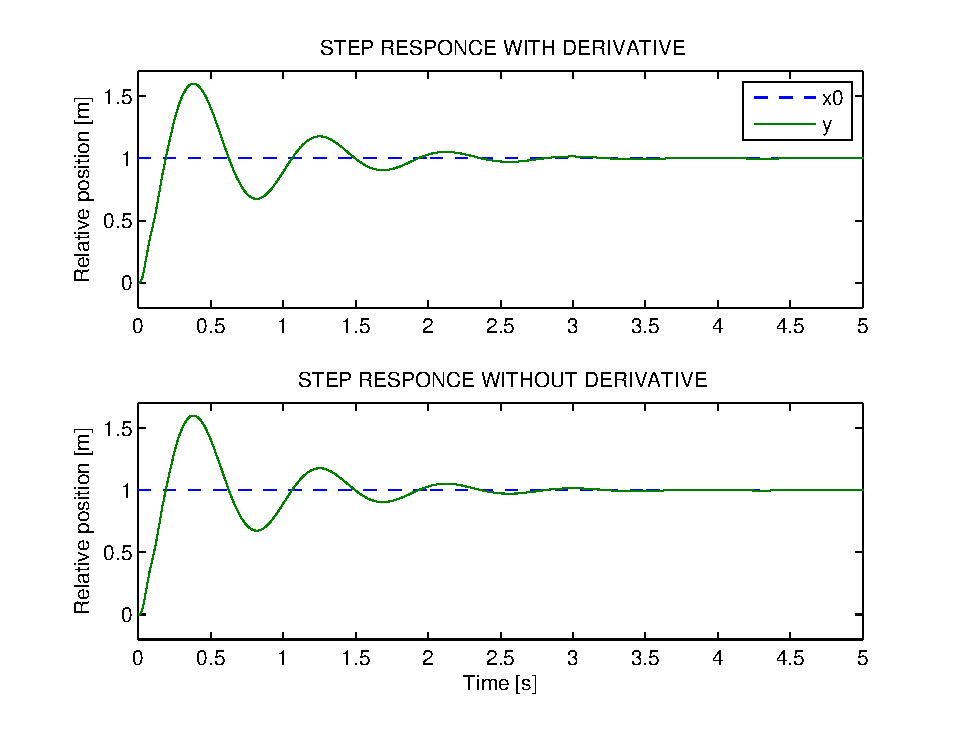
\includegraphics[width=12cm]{../res/img/step_compare.eps}
	\end{center}
	\caption{Odpowiedzi skokowe badanych modeli}
\end{figure}

Jak widać uzyskane odpowiedzi są identyczne, co pozwala założyć, że oba modele
są równoważne. 

\newpage

\subsection{Charakterystyki częstotliwościowe modeli}

Na podstawie wyznaczonego równania stanu \eqref{equ:rstanu} przy pomocy funkcji
\textit{bode} pakietu \textsc{Matlab} wyznaczyłem charakterystyki
częstotliwościowe badanego systemu:

\begin{figure}[!htb]
	\begin{center}
		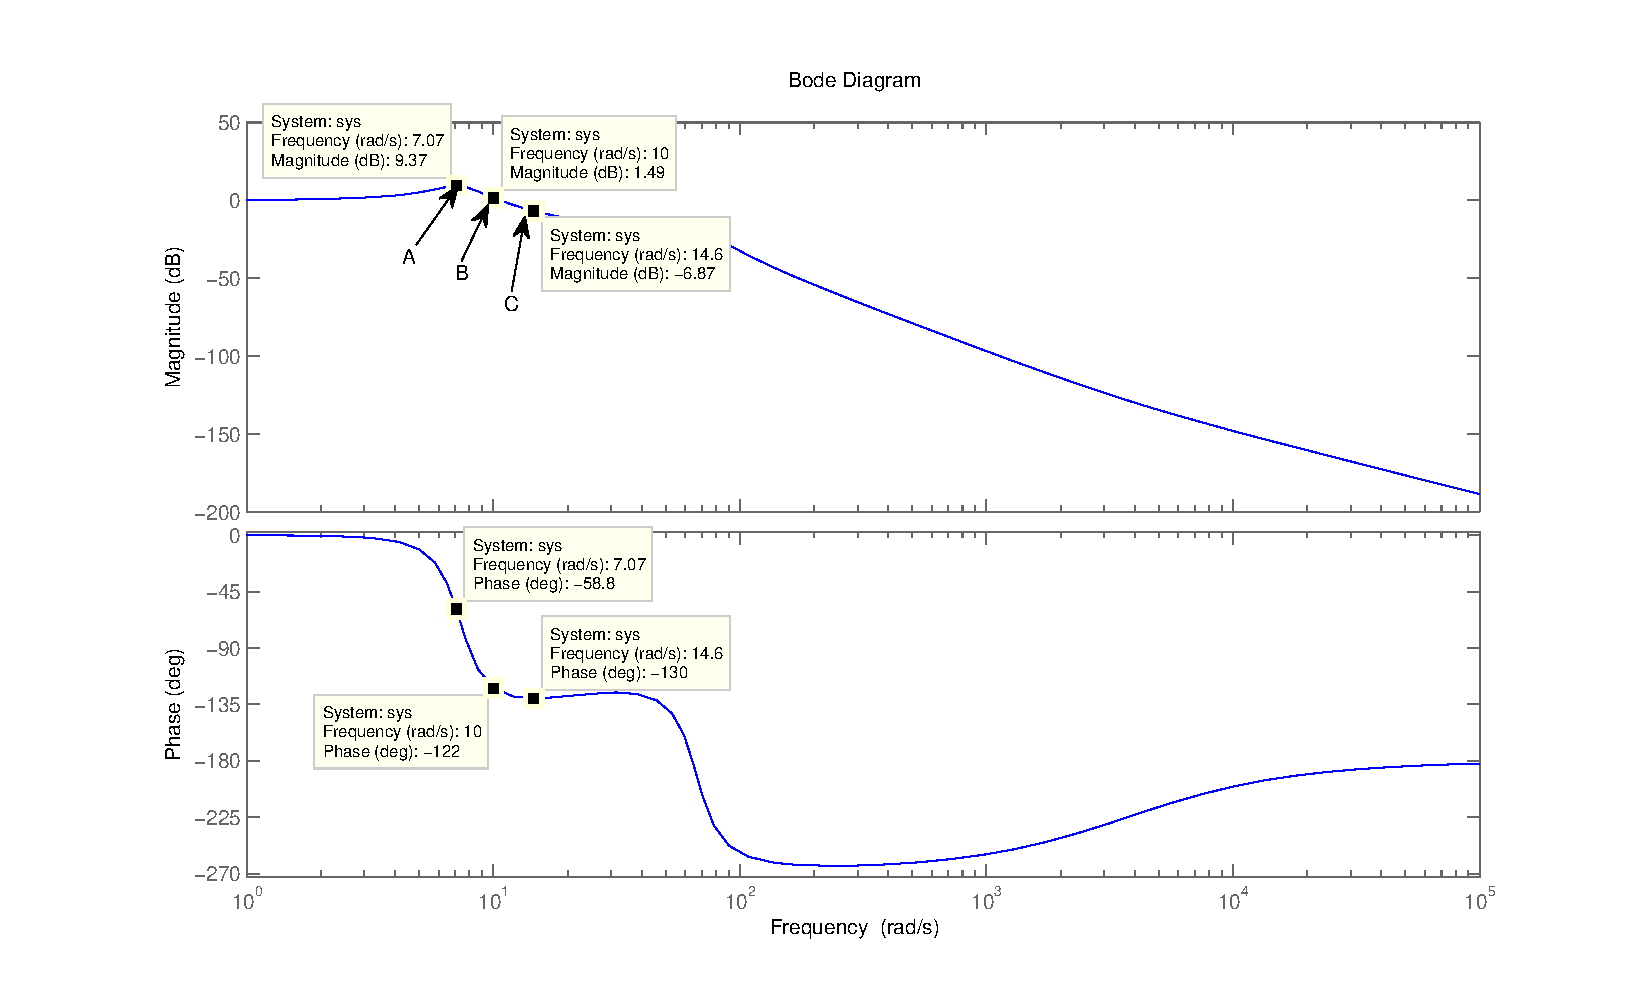
\includegraphics[width=\linewidth]{../res/img/bode.eps}
	\end{center}
	\caption{Charakterystyki Bodego badanego modelu}
	\label{rys:bode}
\end{figure}

Na charakterystykach zostały oznaczone 3 punkty w okolicy częstotliwości dla
której wzmocnienie systemu zaczyna spadać. Dla tych częstotliwości w następnym
podpunkcie zostaną zasymulowane odpowiedzi układu na wymuszający sygnał
prostokątny. 

\newpage

\subsection{Analiza modeli pod kątem częstotliwości sygnału wymuszającego} 

Poniżej przedstawione są odpowiedzi systemu na wymuszenia prostokątne o
częstotliwościach podstawowych zadanych w poprzednim podpunkcie:
 
\begin{figure}[!htb]
	\begin{center}
		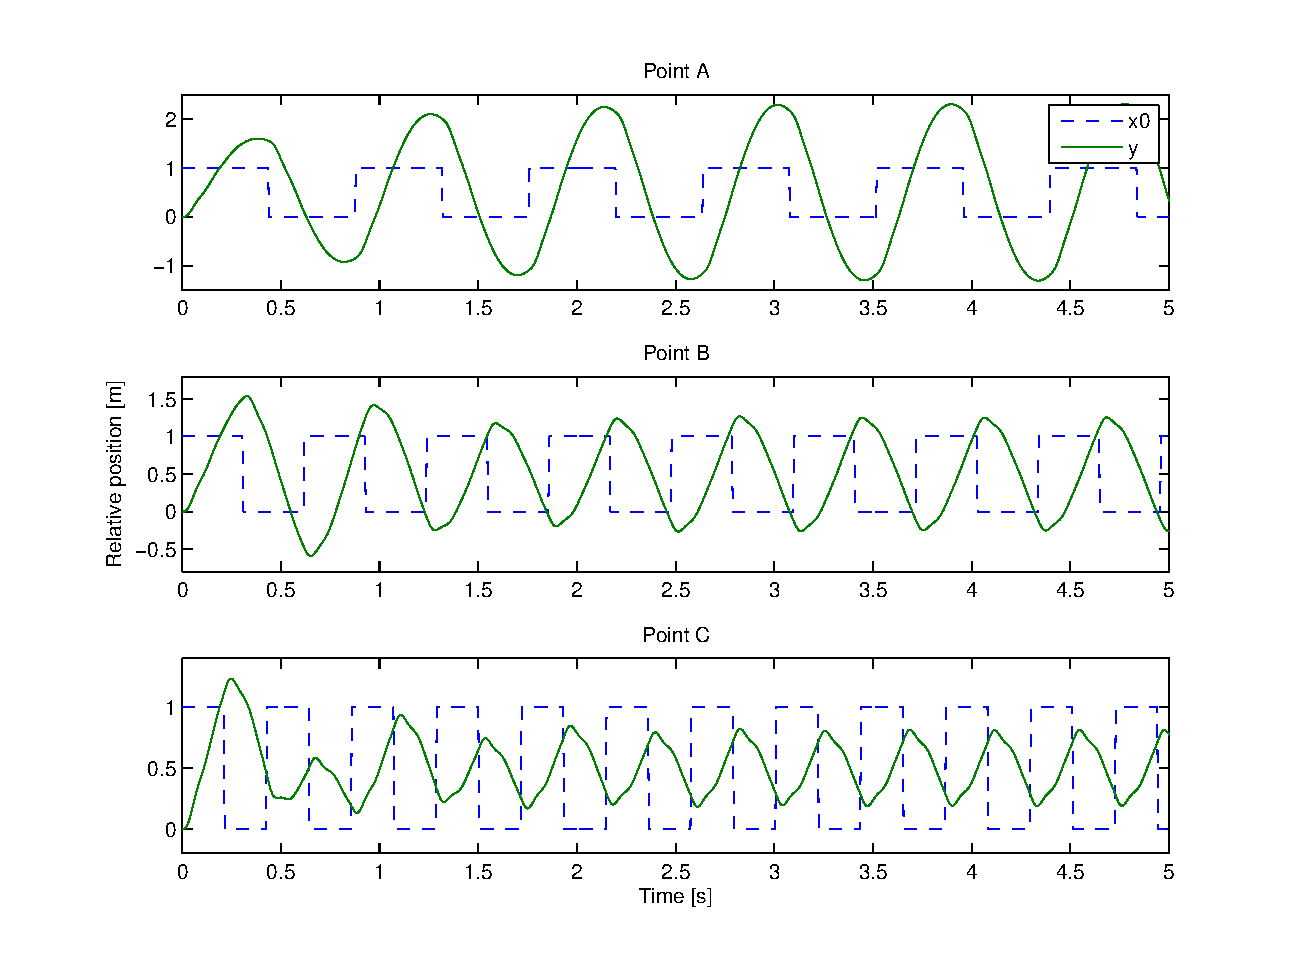
\includegraphics[width=\linewidth]{../res/img/responces.eps}
	\end{center}
	\caption{Odpowiedzi modelu zawieszenia na kilka prostokątnych przebiegów
	nierówności drogi}
\end{figure}

Z uwagi na to, iż utworzone modele są równoważne prezentuję jedynie jeden zestaw
odpowiedzi na wymuszenia.

Obserwując odpowiedzi systemu, można zauważyć, że model zaczyna wykazywać
właściwości tłumiące dopiero od pewnej częstotliwości granicznej. Dla zbadanych
częstości tłumienie widać dopiero dla $\omega=14.6
[\frac{Rad}{\textrm{s}}]$, co zresztą wyraźnie widać na charakterystyce
wzmocnienia Bodego.

\newpage

\subsection{Analiza modeli pod kątem zmiany ich parametrów}

Modelowany system zależy od 6 parametrów, z czego 2 typowo ulegają zmianie, jako
parametry właściwego układu amortyzacji, mianowicie $k_2$ oraz $c_2$. Poniżej
przedstawione są odpowiedzi systemu dla kilku wariantów parametrów amortyzatora
i sprężyny, dla ustalonej częstotliwości wymuszającej
$\omega=7.07[\frac{Rad}{\textrm{s}}]$:

\begin{figure}[!htb]
	\begin{center}
		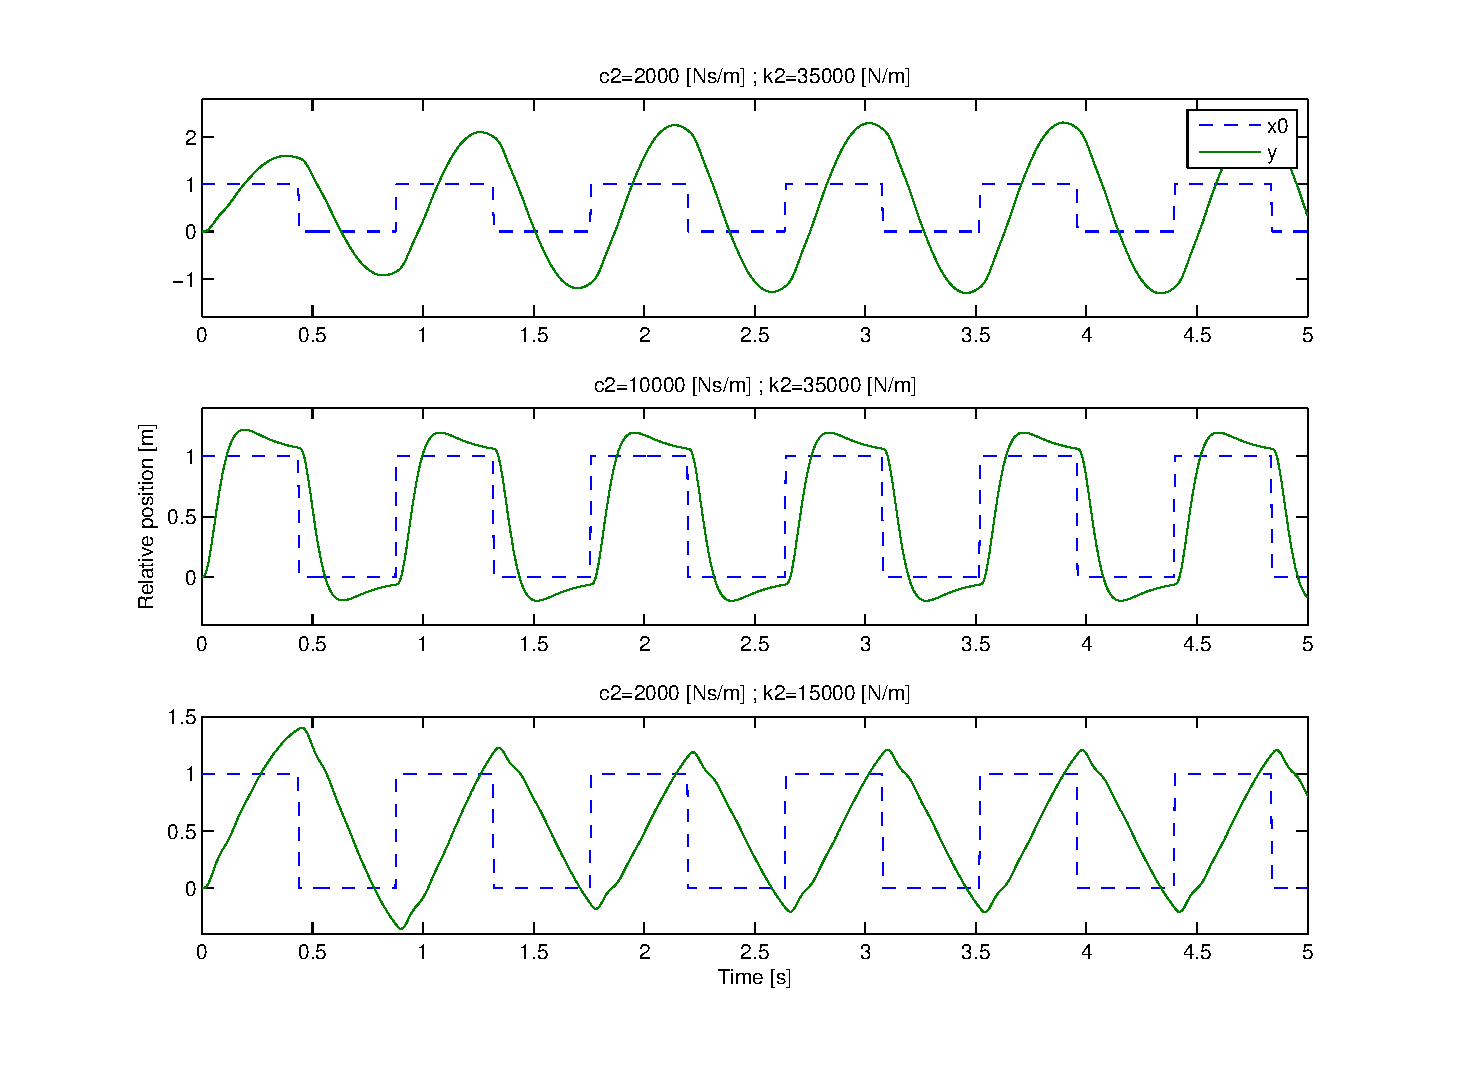
\includegraphics[width=\linewidth]{../res/img/responces_par.eps}
	\end{center}
	\caption{Odpowiedzi modelu zawieszenia na wymuszenie o częstotliwości
	$\omega=7.07[\frac{Rad}{\textrm{s}}]$, dla zmiennych jego parametrów}
\end{figure}

Jak widać zwiększenie wartości współczynnika $c_2$ amortyzatora powoduje
przytłumienie odpowiedzi układu i upodobnienie jej kształtu do kształtu sygnału
wymuszającego, natomiast zmniejszenie wartości współczynnika sprężystości $k_2$
powoduje zwiększenie gwałtowności zmian odpowiedzi podczas skokowych zmian wejścia.

Zachowanie takie jest zgodne z intuicją - im twardszy amortyzator, tym bardziej
odpowiedź karoserii będzie przypominać wymuszenie, natomiast zmniejszenie wpływu
sprężyny spowoduje zanik właściwości łagodzących przebieg odpowiedzi.

\newpage

\section{Wnioski i spostrzeżenia}

Laboratorium polegało na wykonaniu modelu fragmentu zawieszenia samochodu w
pakiecie \textsc{Matlab-Simulink}. W jego trakcie wykonałem 2 implementacje
modelu korzystając z bloków całkujących pakietu \textsc{Simulink}. Uzyskane
wyniki, będące zgodne z intuicją i obserwowanymi w rzeczywistości układami
zawieszeń samochodów, pozwalają stwierdzić, iż wykonane modele są poprawne.

Charakterystyka częstotliwościowa badanego modelu ma charakter dolnoprzepustowy,
toteż jego działanie jest widoczne dopiero dla większych częstotliwości, jednak
są to typowe częstotliwości pracy zawieszenia samochodu, więc jego działanie
jest jak najbardziej poprawne.

\end{document}